\begin{figure}[h]
\begin{center}
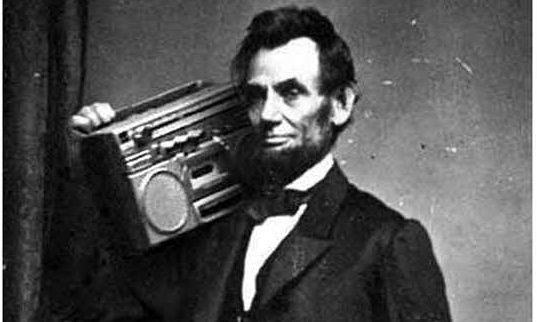
\includegraphics[width=0.6\textwidth] {imagenes/frecuencia.jpeg}
\end{center}
\end{figure}

\subsection{Problema a resolver}
Se tienen una lista de frecuencias con un tiempo de inicio y fin y un costo por transmisión. El problema a resolver consiste en dar un algoritmo que minimice los costos, es decir, que para cada tiempo encuentre la frecuencia con menor costo e indique como ir cambiando de frecuencia acorde pasa el tiempo.

\begin{itemize}
\item Ejemplo: Situación inicial.

\begin{codesnippet}
2
10 1 16
5 6 10
\end{codesnippet}

Aquí se presentan dos señales, la primera tiene costo 10, inicio 1 y fin 16. La segunda tiene costo 5, inicio 6 y fin 10.

En este caso el algoritmo debe elegir la mejor señal para los tiempos 1 al 16.
\item Solución del ejemplo:

\begin{codesnippet}
130
1 1 6
2 6 10
1 10 16
\end{codesnippet}

La solución muestra que lo mejor es usar la primera señal de los tiempos 1 al 6, luego pasar a la segunda del 6 al 10 para, finalmente, retornar a la primer señal del 10 al 16.

El costo total de la transmisión anterior es 130 que es el menor costo posible para el ejemplo.

\end{itemize}

\subsection{Resolución planteada}
La solución planteada utiliza la técnica de \textit{Divide and Conquer}. La idea utilizada está basada en el algoritmo Merge Sort.
Se agregan todas las señales recibidas a un vector y luego se llama a una función que se queda con dos problemas de la mitad de tamaño en cada paso, se llama a la misma recursivamente hasta llegar al caso base y luego se unen las soluciones en un único vector con la solución de la siguiente manera:


Creo un iterador para cada uno de los vectores (los llamamos vector izq y der):

\begin{codesnippet}
int izq_it <- 0
int der_it <- 0
\end{codesnippet}


Mientras alguno de los iteradores sea menor al tamaño del vector que itera me fijo
cual de los dos elementos a los que apuntan los iteradores tiene menor principio
y llamo a una funcion auxiliar que los ordenará.

\begin{codesnippet}
izq y der son Vector<Signal>
    donde Signal es tupla <numero:int, costo:int, principio:int, final:int>
Mientras izq_it < |izq| y der_it < |der| hacer:
    Si izq[izq_it].principio <= der[det_it].principio:
        mergeAux(izq, der, izq_it, der_it)
    Sino
        mergeAux(der, izq, der_it, izq_it)
    Fin if
Fin ciclo
\end{codesnippet}    


Una vez que sale del ciclo, significa que al menos uno de los vectores fue recorrido
completamente, por eso agrego los elementos restantes al vector solución:

\begin{codesnippet}
Mientras izq_it < |izq| hacer:
    result.agregarAlFinal(izq[izq_it])
    izq_it <- izq_it + 1
Fin ciclo

Mientras der_it < |der| hacer:
    result.agregarAlFinal(der[der_it])
    der_it <- der_it + 1
Fin ciclo
\end{codesnippet}    


\vspace{1em}
Pasamos a mostrar como la función auxiliar mergeAux compara dos señales dadas. Llamaremos \textit{primera} a la que tiene menor principio y \textit{segunda} a la que tiene mayor principio. Se contemplan los siguientes casos:

\begin{itemize}
	\item Si el costo de la \textit{primera} es menor o igual al de la \textit{segunda}:
        \begin{itemize}
            \item Si el principio de la segunda es mayor al final de la primera, entonces agrego la primera al resultado.
            \item Si el principio de la segunda es menor o igual al final de la primera y el final de la primera es menor al final de la segunda. Entonces, agrego la primera al resultado y le pongo como nuevo principio a la segunda el final de la primera.
            \item Si el principio de la segunda es menor o igual al final de la primera y el final de la primera es mayor o igual al final de la segunda. Entonces desestimo la segunda señal.
        \end{itemize}

	\item Si el costo de la primera es mayor al de la segunda:
Guardo una variable int auxiliar (de ahora en adelante aux) con el final de la primera
        \begin{itemize}
            \item Si el principio de la segunda es menor o igual al final de la primera y el final de la primera es mayor al principio, entonces le pongo como fin a la primera el principio de la segunda y la agrego al resultado. Si el fin de la segunda es menor que aux, modifico la primera poniendole como principio el final de la segunda y como final a aux y no aumento el iterador.
            \item Si el principio de la segunda es menor o igual al final de la primera y el final de la primera es menor o igual al principio, entonces le pongo como fin a la primera el principio de la segunda y desestimo el resultado.
            \item Si el principio de la segunda es mayor al final de la primera, entonces agrego la primera al resultado.
        \end{itemize}
\end{itemize}

% \begin{codesnippet}

% menor , mayor y result son puntero(Vector<Signal>) 
% donde Signal es tupla <numero:int,costo:int,principio:int,final:int>

% i,j son puntero(int)

% mergeAux(Vec& menor, Vec& mayor, int& i, int& j,Vec& result){
%     bool flag <- false;
    

%     if(menor[i].costo <= mayor[j].costo)
%         if(mayor[j].principio <= menor[i].fin)
%             mayor[j].principio <- menor[i].fin
%         end if
%         if(mayor[j].principio >= mayor[j].fin) {
%             j <- j + 1
%             flag <- true
%         end if
%         if(!flag) {
%             result.agregarAlFinal(menor[i])
%             i <- i + 1
%         else
%             flag <- false
%         end if
%     else
%         int aux <- menor[i].fin;
%         if(mayor[j].principio <= menor[i].fin) {
%             menor[i].fin <- mayor[j].principio
%         end if
%         if(menor[i].fin > menor[i].principio) {
%             result.agregarAlFinal(menor[i])
%         end if
%         if(mayor[j].fin < aux) {
%             menor[i].principio <- mayor[j].fin
%             menor[i].fin <- aux
%         else
%             i++;
%         end if
%     end if
% }
% \end{codesnippet} 



\subsection{Complejidad propuesta}

Analizamos la complejidad usando Teorema Maestro\footnote{Teorema Maestro \url{http://es.wikipedia.org/wiki/Teorema_maestro}}:. En cada paso nos quedamos con dos subproblemas que tienen la mitad de tamaño que el original, así que a = 2 y c = 2. Además de la recursión, se unen los resultados. Para esto llamamos a la función merge, que realiza como máximo $2n-1$ operaciones(*) con n el tamaño de la entrada. Esto tiene complejidad lineal en la cantidad de elementos del arreglo. Más allá de esto, se hace una cantidad constante de comparaciones y asignaciones, por lo que podemos decir que f(n)  $\in$  $\Theta$ 
(n). No podríamos usar el primer caso del teorema, porque $n^{\log_2 2-\epsilon}$ = $n^{1 - \epsilon}$ , y no es cierto que f(n) $\in$  $\Theta$ ($n^{1 - \epsilon}$ ). En cambio, podemos usar el segundo caso, porque como ya dijimos f(n) $\in$ $\Theta$ (n). Reemplazando, obtenemos T(n) $\in$
 $\Theta$ ( $n^{\log_2 2}$  $log (n)$), o sea T(n) $\in$  $\Theta$ ($n$  $log (n)$).
 \\
 
 (*)
 Veamos por inducción que el peor caso es 2n-1:
 \\
 
 Primero notemos que la función mergeAux solo hace una cantidad de comparaciones y asignaciones constantes, o sea, que tiene complejidad O(1).
\begin{itemize} 
\item Caso base n=1


Si n=1 la función merge no entrará en el primer ciclo ya que uno de los dos vectores a comparar tendrá tamaño 0 y tanto izq_it como der_it son 0. Por ende, solo agregará la única señal disponible al resultado realizando una cantidad constante de operaciones. Como 2n-1 = 2-1 = 1 se cumple.
 
\item Paso Inductivo

Supongamos que vale para n. Veamos que vale para n+1. Si tenemos n+1 señales, entonces la función entra en el ciclo de la función merge al menos una vez. Esto significa que entra en la función mergeAux al menos una vez. Viendo la función mergeAux podemos observar los posibles casos al comparar dos señales:

Llamaremos \textit{primera} a la que tiene menor principio y \textit{segunda} a la que tiene mayor principio.

\begin{itemize}
\item Que la primera tenga menor costo que la segunda y menor final que el principio de la segunda.\\
Ejemplo:

\begin{codesnippet}
1 1 4
2 5 6
\end{codesnippet}

En este caso se llamará a mergeAux una vez, se agregará la primera señal al resultado y se aumentará el iterador i, resultando así un vector de tamaño n.

\item Que la primera tenga menor o igual costo que la segunda y que la segunda esté completamente contenida dentro de la primera.\\
Ejemplo:

\begin{codesnippet}
1 1 4
2 2 3
\end{codesnippet}

En este caso se llamará a mergeAux una vez, se aumentará el iterador j, resultando asi un vector de tamaño n.

\item Que la primera tenga menor o igual costo que la segunda y menor final que la segunda.\\
Ejemplo:

\begin{codesnippet}
1 1 4
2 3 6
\end{codesnippet}

En este caso se llamará a mergeAux una vez, se le pondrá como comienzo a la segunda el final de la primera. Luego, se agregará la primera al resultado y se aumentará el iterador, resultando así un vector de tamaño n.

\item Que la primera tenga mayor costo que la segunda y mayor final que el final de la segunda.\\
Ejemplo:

\begin{codesnippet}
2 1 4
1 2 3
\end{codesnippet}

En este caso se llamará a mergeAux una vez, se guardará el fin de la primera en una variable auxiliar. Luego, se pondrá como fin de la primera el comienzo de la segunda y se agregará la primera al resultado. Después, se le pondrá como principio a la primera el fin de la segunda y como fin el valor guardado en la variable auxiliar. Como no aumentaron los iteradores, se llamará de nuevo a la función. En el ejemplo anterior con los siguientes valores ahora:

\begin{codesnippet}
2 3 4
1 2 3
\end{codesnippet}

Ahora la función es equivalente al primer ejemplo de la esta lista. Por lo que se agregará una al reultado y se aumentara un iterador resultando así una función de tamaño n.
En este caso se llamó dos veces a la función mergeAux.

\item Que la primera tenga mayor costo que la segunda y menor final que el principio de la segunda.\\
Ejemplo:

\begin{codesnippet}
2 1 4
1 5 6
\end{codesnippet}

En este caso se llamará a mergeAux una vez, se agregará la primera al resultado y se aumentará el iterador i, resultando así un vector de tamaño n.

\item Que la primera tenga mayor costo que la segunda y mayor final que el principio de la segunda.\\
Ejemplo:

\begin{codesnippet}
2 1 4
1 3 6
\end{codesnippet}

En este caso se llamará a mergeAux una vez, se le pondrá a la primera como fin el principio de la mayor, se agregará esta al resultado y se aumentará el iterador i, resultando así un vector de tamaño n.

\end{itemize}

Como podemos ver, en todos los casos anteriores salvo en uno se llama una vez sola a la función mergeAux. En el peor caso esta se llama dos veces o sea, con costo 2*O(1). Veamos entonces que 2(n+1)-1 = 2n+2-1 = 2n+1. En el peor caso se llama a la función dos veces con costo O(1) y luego queda un vector de tamaño n, que por hipotesis inductiva tiene costo 2n-1.

Ahora 2n-1+2 = 2n+1 = 2(n+1)-1. Entonces queda demostrado.

 
\end{itemize} 
 
 

\newpage
\subsection{Implementación en C++}

\lstinputlisting[language=C++]{codigo/ej2.cpp}



\subsection{Experimentación computacional}
La función que utilizamos para llevar a cabo las mediciones fue \texttt{std::clock}\footnote{Referencia \url{http://en.cppreference.com/w/cpp/chrono/c/clock}}. La unidad temporal que utilizamos para este ejercicio fue de nanosegundos.
La complejidad teórica calculada es de $\mathcal{O}(n*log(n))$

\subsubsection{Experimentación con instancias aleatorias}
Para generar las instancias aleatorias utilizamos la función \texttt{std::rand}\footnote{Referencia \url{http://en.cppreference.com/w/cpp/numeric/random/rand}} con determinados intervalos de valores para la variables, para obtener instancias coherentes. El detalle de intervalos es el siguiente:
\begin{itemize}
	\item Cantidad de muestras: 100
	\item Cantidad de frecuencias ($n$): de 1 a 3000
    \item Costos ($P$): 1 $\leq P \leq$ 10.000
    \item Para los inicios y finales se verifico que el final sea mayor al inicio en cada frecuencia
\end{itemize}

Se generaron 100 muestras. Para cada muestra se generaron instancias aleatorias de tamaños 1 a 3000.
Luego se tomo el promedio de tiempos para cada tamaño en las 100 muestras

\begin{figure}[H]
        \centering
        \begin{subfigure}[b]{0.5\textwidth}
                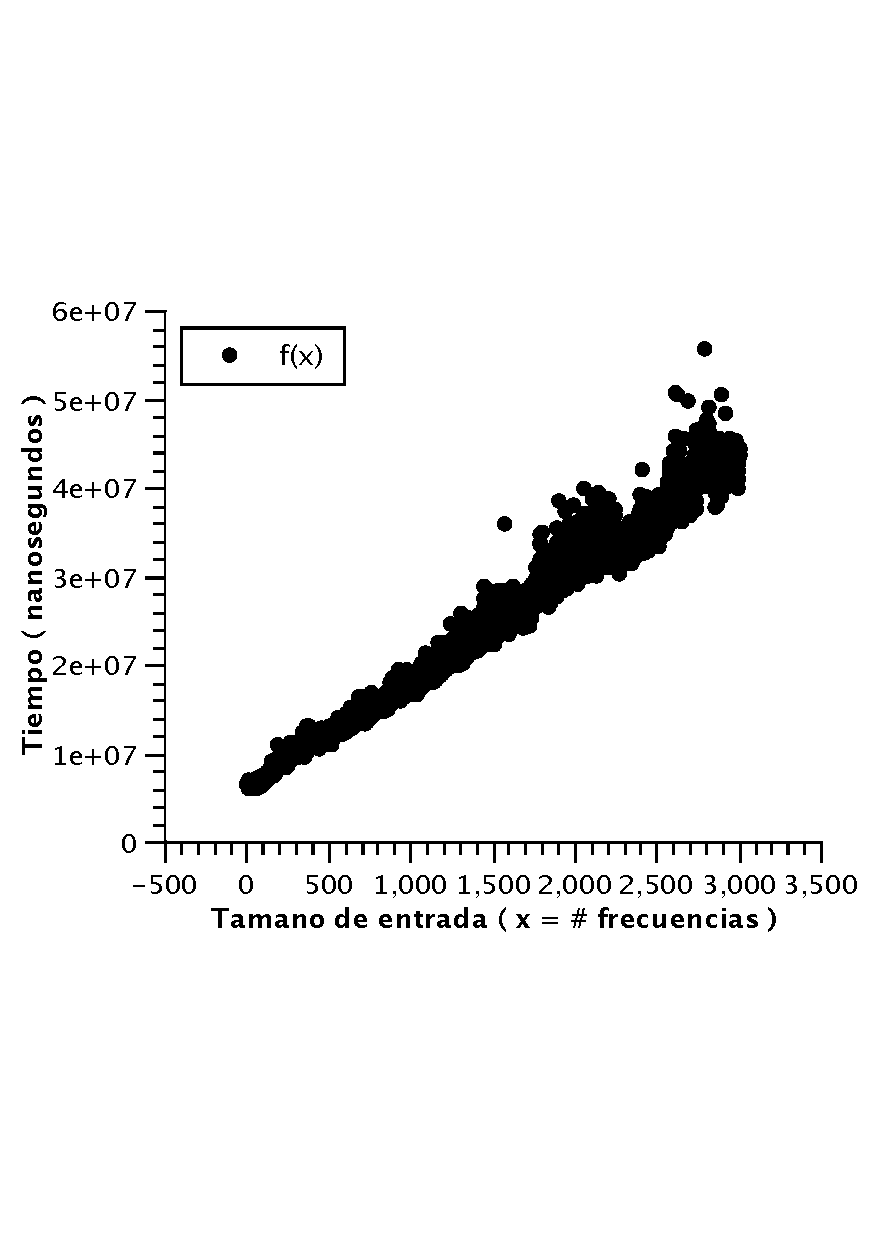
\includegraphics[width=\textwidth]{imagenes/af-rand-nlogn.pdf}
                \caption{Tiempos sin procesar}
        \end{subfigure}%
        ~ %add desired spacing between images, e. g. ~, \quad, \qquad, \hfill etc.
          %(or a blank line to force the subfigure onto a new line)
        \begin{subfigure}[b]{0.5\textwidth}
                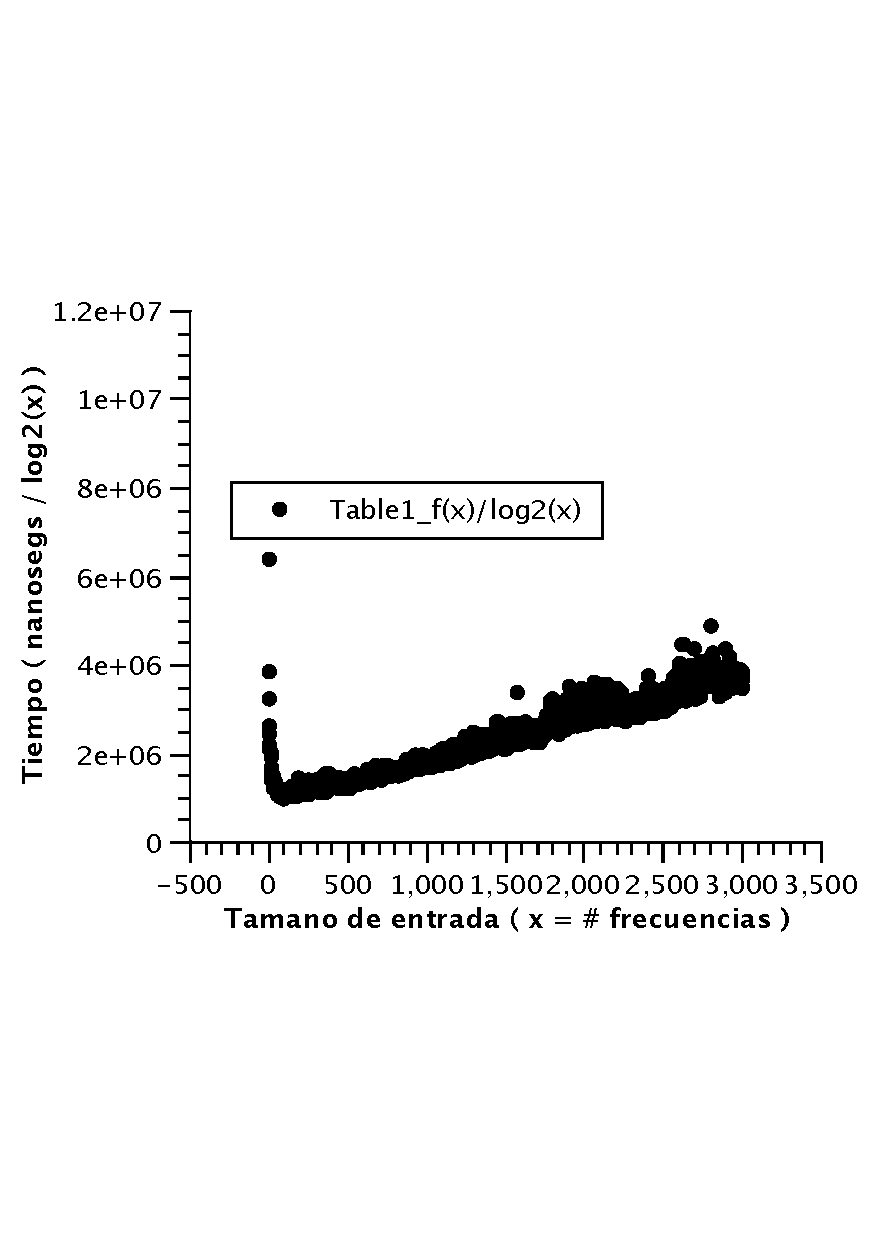
\includegraphics[width=\textwidth]{imagenes/af-rand-lineal.pdf}
                \caption{Logaritmo a la figura (a)}
        \end{subfigure}
        
        \begin{subfigure}[b]{0.5\textwidth}
                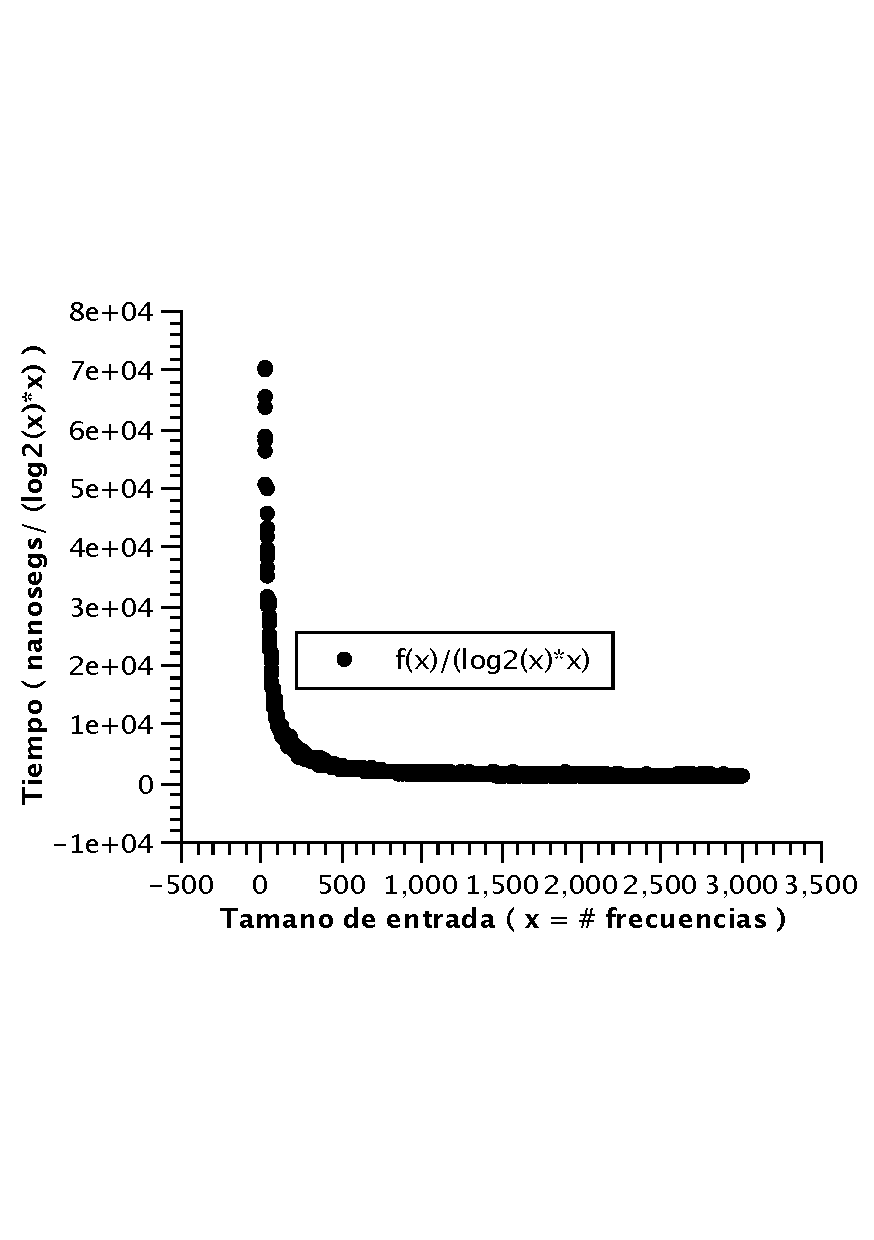
\includegraphics[width=\textwidth]{imagenes/af-rand-const.pdf}
                \caption{Dividiendo por x la figura (b)}
        \end{subfigure}
        \caption{}
\end{figure}



A continuación, adjuntamos una tabla con los ultimos 20 valores obtenidos en este último paso, teniendo en cuenta que los casos fueron previamente ordenados segun el tamaño ($n$):

\begin{table}[H]
\parbox{0.3\textwidth}{
    \begin{tabular}{ | l | l | l | l |}
    \hline
Tamano($n$) & Tiempo($t$) & $t / log(n)$ & $t / n*log(n)$ \\ \hline
2,980 & 41,823,717 & 3,623,894.53913547 & 1,216.07199299848 \\ \hline
2,981 & 42,205,634 & 3,656,833.08407709 & 1,226.713547157695 \\ \hline
2,982 & 41,379,610 & 3,585,113.377975757 & 1,202.251300461354 \\ \hline
2,983 & 42,125,330 & 3,649,569.318887776 & 1,223.456023763921 \\ \hline
2,984 & 45,341,672 & 3,928,055.705472136 & 1,316.372555453129 \\ \hline
2,985 & 40,887,769 & 3,542,055.278169351 & 1,186.618183641324 \\ \hline
2,986 & 42,795,296 & 3,707,146.720857472 & 1,241.509283609334 \\ \hline
2,987 & 43,971,377 & 3,808,865.466588621 & 1,275.147461194717 \\ \hline
2,988 & 41,832,598 & 3,623,449.707752226 & 1,212.667238203556 \\ \hline
2,989 & 41,938,501 & 3,632,470.907368039 & 1,215.279661213797 \\ \hline
2,990 & 41,182,479 & 3,566,839.555032387 & 1,192.922928104477 \\ \hline
2,991 & 43,525,502 & 3,769,612.695656072 & 1,260.318520781034 \\ \hline
2,992 & 42,113,000 & 3,647,127.818332012 & 1,218.959832330218 \\ \hline
2,993 & 42,931,618 & 3,717,867.670108657 & 1,242.187661245792 \\ \hline
2,994 & 43,479,759 & 3,765,179.403366345 & 1,257.574951024163 \\ \hline
2,995 & 42,626,427 & 3,691,130.148415261 & 1,232.430767417449 \\ \hline
2,996 & 42,621,659 & 3,690,563.361166947 & 1,231.830227358794 \\ \hline
2,997 & 40,046,500 & 3,467,438.573756513 & 1,156.969827746584 \\ \hline
2,998 & 40,993,661 & 3,549,300.88989128 & 1,183.88955633465 \\ \hline
2,999 & 44,504,732 & 3,853,134.875349259 & 1,284.806560636632 \\ \hline
3,000 & 43,832,216 & 3,794,751.699991118 & 1,264.917233330373 \\ \hline
    \end{tabular}
}
\end{table}

A partir de la información suministrada, podemos observar que, en el gráfico (a) las mediciones tienden a algo un poco más grande que lineal. Al dividirlo por logaritmo de n a estas (b) se observa que el gráfico tiende a ser lineal. Por último en (c) se lo divide además de por logaritmo de n, por n y el gráfico que arroja es constante y mayor a 0. Por lo que podemos concluir que la complejidad de $\mathcal{O}(n*log(n))$ se condice con nuestra predicción de complejidad.

\subsubsection{Experimentación con instancias particulares}

Como quedo demostrado en la justificación de la complejidad teórica, el peor caso ocurre cuando al comparar dos frecuencias la de menor costo esta completamente contenida dentro de la de mayor costo, en este caso, la salida termina teniendo 2n-1 señales. Generamos una muestra de peor caso de tamaños 1 a 3000 de la siguiente manera:
\begin{itemize}
	\item El costo de la primer frecuencia es 3001
	\item El comienzo de la primer frecuencia es 1
    \item El final de la primer frecuencia es 6001
    \item Cada frecuencia que se agrega disminuye en 1 el costo, aumenta en 1 el comienzo y disminuye en 1 el final
\end{itemize}


\begin{figure}[H]
        \centering
        \begin{subfigure}[b]{0.5\textwidth}
                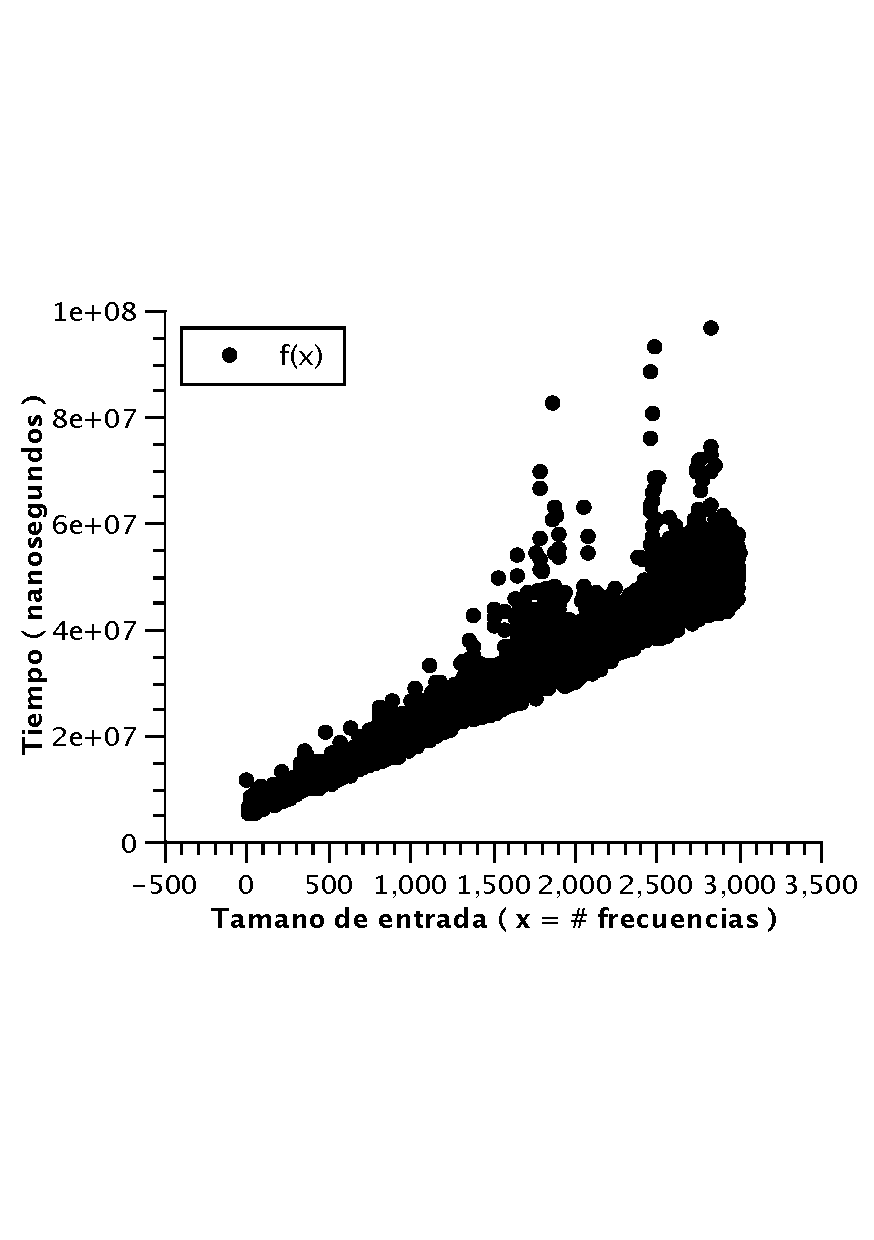
\includegraphics[width=\textwidth]{imagenes/af-wc-nlogn.pdf}
                \caption{Tiempos sin procesar}
        \end{subfigure}%
        ~ %add desired spacing between images, e. g. ~, \quad, \qquad, \hfill etc.
          %(or a blank line to force the subfigure onto a new line)
        \begin{subfigure}[b]{0.5\textwidth}
                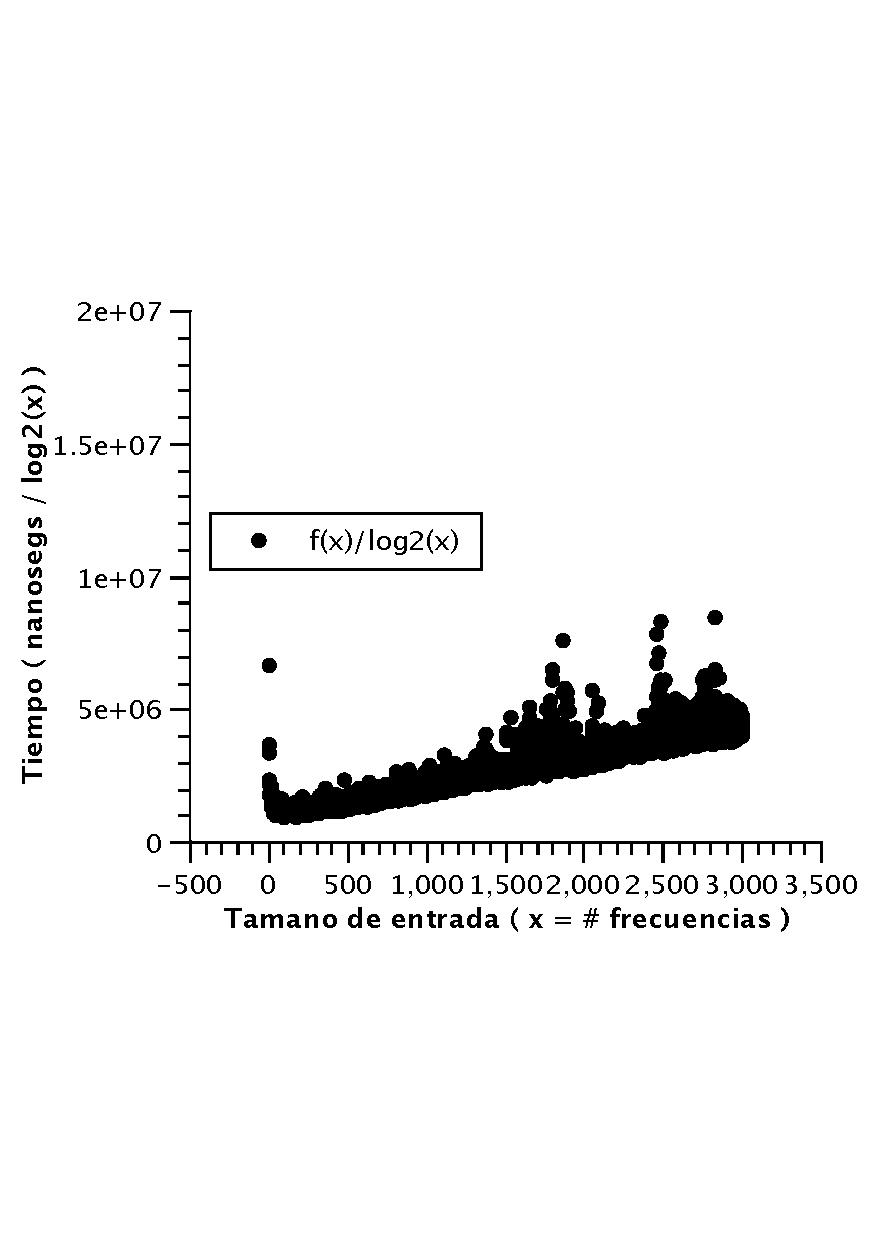
\includegraphics[width=\textwidth]{imagenes/af-wc-lineal.pdf}
                \caption{Logaritmo a la figura (a)}
        \end{subfigure}
        
        \begin{subfigure}[b]{0.5\textwidth}
                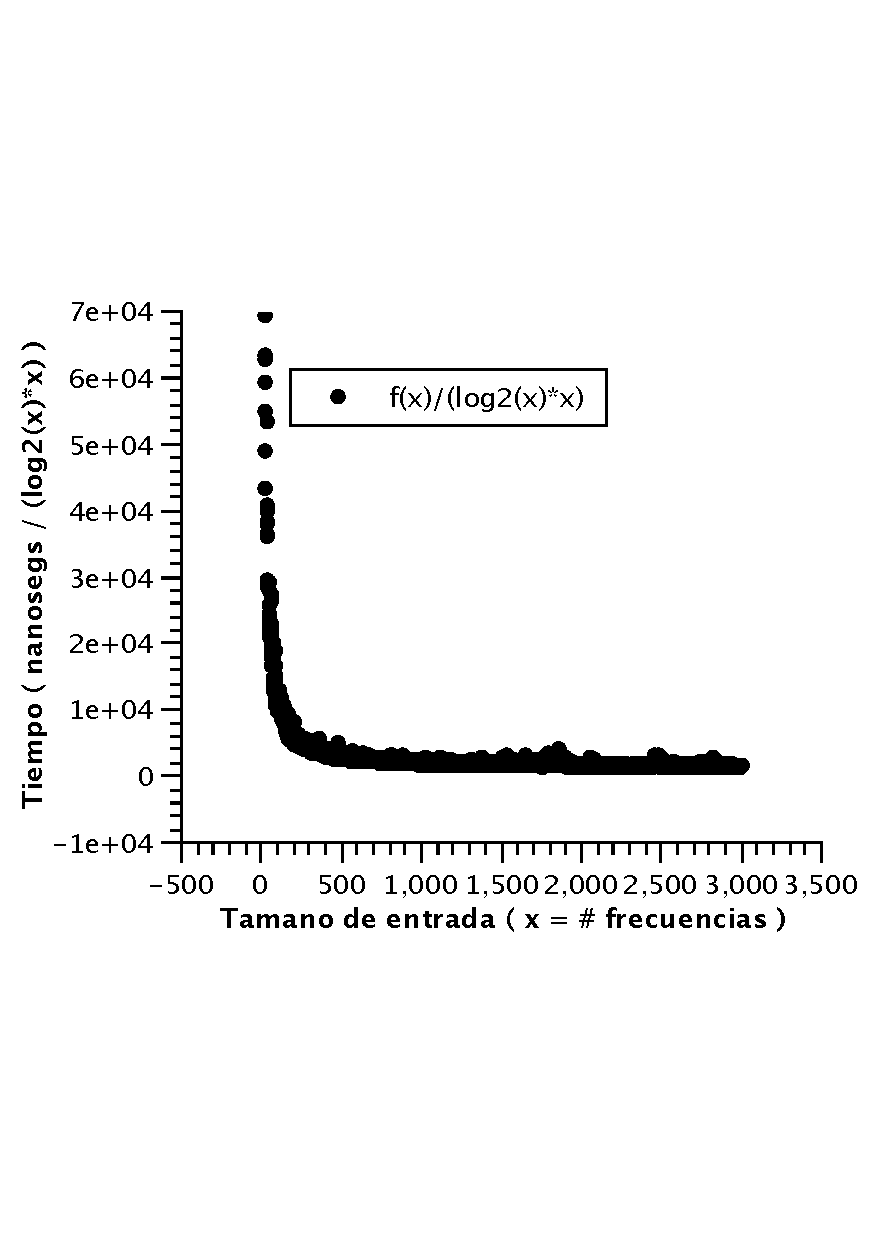
\includegraphics[width=\textwidth]{imagenes/af-wc-const.pdf}
                \caption{Dividiendo por x la figura (b)}
        \end{subfigure}
        \caption{}
\end{figure}



A continuación, adjuntamos una tabla con los ultimos 20 valores obtenidos en este último paso, teniendo en cuenta que los casos fueron previamente ordenados segun el tamaño ($n$):

\begin{table}[H]
\parbox{0.3\textwidth}{
    \begin{tabular}{ | l | l | l | l |}
    \hline
Tamano($n$) & Tiempo($t$) & $t / log(n)$ & $t / n*log(n)$ \\ \hline
2,980 & 47,188,711 & 4,088,754.524179232 & 1,372.065276570212 \\ \hline
2,981 & 48,174,802 & 4,174,021.169127874 & 1,400.208376091202 \\ \hline
2,982 & 47,537,404 & 4,118,622.264314194 & 1,381.161054431319 \\ \hline
2,983 & 50,090,561 & 4,339,644.926021389 & 1,454.792130748035 \\ \hline
2,984 & 50,262,066 & 4,354,321.012249329 & 1,459.222859332885 \\ \hline
2,985 & 50,960,628 & 4,414,654.205912404 & 1,478.946132633971 \\ \hline
2,986 & 51,054,247 & 4,422,579.162716796 & 1,481.104876998257 \\ \hline
2,987 & 58,162,121 & 5,038,088.62161512 & 1,686.671784939779 \\ \hline
2,988 & 53,436,807 & 4,628,581.344801059 & 1,549.056674966887 \\ \hline
2,989 & 57,760,600 & 5,002,889.805053413 & 1,673.767080981403 \\ \hline
2,990 & 50,334,133 & 4,359,469.874376941 & 1,458.016680393625 \\ \hline
2,991 & 52,002,106 & 4,503,745.849466659 & 1,505.765914231581 \\ \hline
2,992 & 55,619,141 & 4,816,805.175903654 & 1,609.894778042665 \\ \hline
2,993 & 53,321,719 & 4,617,647.88796729 & 1,542.815866343899 \\ \hline
2,994 & 49,501,380 & 4,286,628.55316679 & 1,431.739663716362 \\ \hline
2,995 & 48,025,112 & 4,158,615.939924299 & 1,388.519512495592 \\ \hline
2,996 & 51,954,186 & 4,498,656.781775029 & 1,501.554333035724 \\ \hline
2,997 & 51,590,387 & 4,466,969.595815528 & 1,490.48034561746 \\ \hline
2,998 & 45,924,717 & 3,976,240.104930008 & 1,326.297566687795 \\ \hline
2,999 & 54,525,123 & 4,720,681.230346652 & 1,574.085105150601 \\ \hline
    \end{tabular}
}
\end{table}



A partir de la información suministrada, podemos observar que, en el gráfico (a) las mediciones tienden a algo un poco más grande que lineal. Al dividirlo por logaritmo de n a estas (b) se observa que el gráfico tiende a ser lineal. Por último en (c) se lo divide además de por logaritmo de n, por n y el gráfico que arroja es constante y mayor a 0. Por lo que podemos concluir que la complejidad de $\mathcal{O}(n*log(n))$ se condice con nuestra predicción de complejidad.